\documentclass[12pt,compress]{beamer}
\usepackage{amsmath}
\usepackage{cmbright}
\usepackage{url}
\usepackage{ucs}
\usepackage[utf8x]{inputenc}
\usepackage[ngerman]{babel}
\usepackage{bbm}
\usepackage{ulem}
\usepackage{multicol}
\usepackage{comment}
\usepackage{setspace}
\usepackage{color}
\usepackage{movie15}
\usepackage{hyperref}
\usepackage{bookman}

\usetheme{Boadilla}
\setbeamertemplate{footline}%{infolines theme}

\usecolortheme{lily}
\usefonttheme{serif}
\useinnertheme{circles}
\setbeamercovered{transparent}
\beamertemplatenavigationsymbolsempty

\definecolor{darkgreen}{rgb}{0,0.5,0}

\hypersetup{
    bookmarks=true,
    unicode=true,
    pdftoolbar=true,
    pdfmenubar=true,
    pdffitwindow=false,
    pdfstartview={FitH},
    pdftitle={Klassisches Chaos und Poincaré-Schnitte},
    pdfauthor={Michael Hartmann},
    pdfsubject={Vortrag über klassisches Chaos in hamiltonschen Systemen am Beispiel des Doppelpendels},
    pdfcreator={vim},
    pdfproducer={pdflatex},
    pdfkeywords={Doppelpendel} {Chaos} {Poincare},
    pdfnewwindow=true,
    colorlinks=true,
    linkcolor=black,
    citecolor=green,
    filecolor=magenta,
    urlcolor=darkgreen
}



\title{Was ist Chaos? }
%\subtitle{Einführung am Beispiel des Doppelpendels}
\institute{Theoretische Physik I}
\author{Michael Hartmann}
\date{18. November 2015}


\titlegraphic{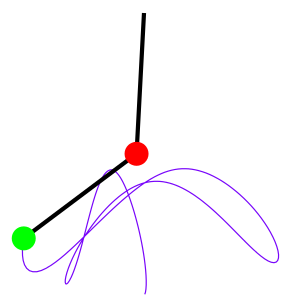
\includegraphics[scale=0.4]{images/title.png}}


\begin{document}

\begin{frame}
    \titlepage
\end{frame}


\section{Was ist ein Doppelpendel?}


\frame {
    \frametitle{Was ist ein Doppelpendel?}

    \begin{minipage}[b]{0.4\textwidth} 
    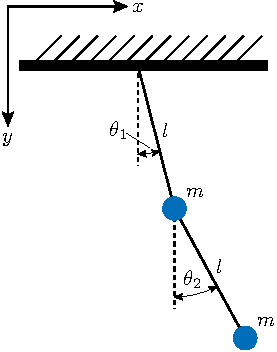
\includegraphics[scale=1]{images/sketch.pdf}
    
    \end{minipage}
    \hfill
    \begin{minipage}[b]{0.4\textwidth}
    \begin{align}
    \nonumber
    x_1 &= l \sin\theta_1 \\
    \nonumber
    y_1 &= -l \cos\theta_1 \\
    \nonumber
    x_2 &= l \sin\theta_1 + l \sin\theta_2 \\
    \nonumber
    y_2 &= -l \cos\theta_1 - l \cos\theta_2
    \end{align}
    \end{minipage}
}

\frame {
    \frametitle{Was ist ein Doppelpendel?}

    \begin{center}
    \includemovie[poster,autoplay,controls=true]{7.5cm}{7.5cm}{videos/pendulum.mp4}
    \end{center}
}

\frame {
    \frametitle{Wovon hängt die Bewegung ab?}

    \only<2>
    {
    Parameter:
    \begin{itemize}
    \item Massen $m_1$, $m_2$
    \item Längen $l_1$, $l_2$
    \item Erdbeschleunigung $g$
    \end{itemize}

    \vfill

    Zustand:
    \begin{itemize}
    \item Winkel $\theta_1$, $\theta_2$
    \item Winkelgeschwindigkeiten $\dot \theta_1$, $\dot \theta_2$
    \end{itemize}
    }
}

\frame {
    \frametitle{Phasenraum}

    \only<1>
    {
    \begin{itemize}
    \item Menge aller möglichen Zustände eines physikalischen Systems
    \item Zustand: Punkt im Phasenraum
    \item Trajektorien können sich nicht schneiden
    \end{itemize}

    \vfill

    Beispiel: Pendel
    \begin{center}
    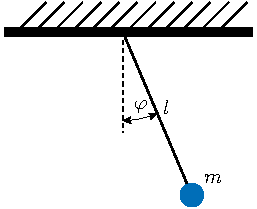
\includegraphics[scale=1]{images/pendulum.pdf}
    \end{center}
    }

    \only<2>
    {
    Beispiel Pendel:

    \begin{center}
    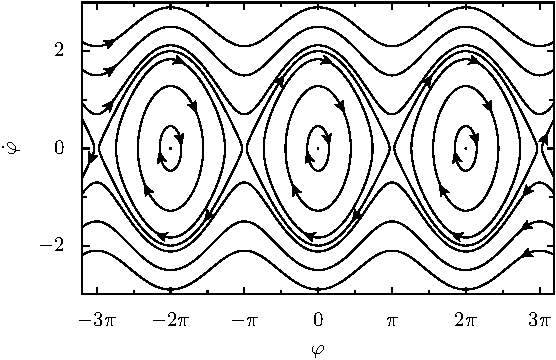
\includegraphics[scale=1]{plots/phasespace.pdf}
    \end{center}
    }

    \only<3>
    {
    Für das Doppelpendel:
    \begin{itemize}
    \item 4 Freiheitsgrade:
    \begin{itemize}
    \item 2 Winkel $\theta_1$, $\theta_2$
    \item 2 Geschwindigkeiten $\dot \theta_1$, $\dot \theta_2$
    \end{itemize}
    \item Energieerhaltung: Trajektorien auf Hyperfläche eingeschränkt
    \item Poincaré-Schnitt: Reduktion auf zwei Dimensionen ohne Verlust an Information
    \end{itemize}
    }
}

\frame {
    \frametitle{Poincaré-Schnitte}

    \only<1>
    {
    \begin{center}
    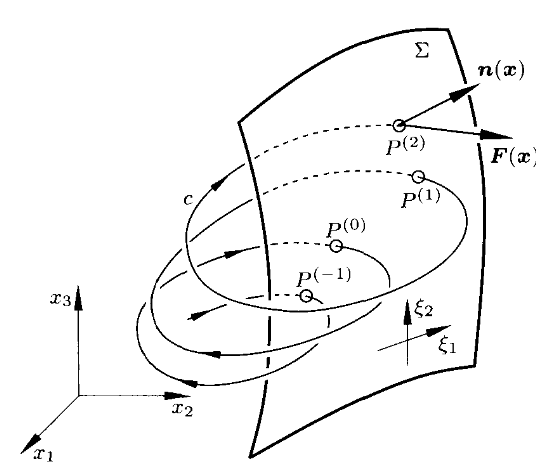
\includegraphics[scale=0.45]{images/poincare_idea.png}
    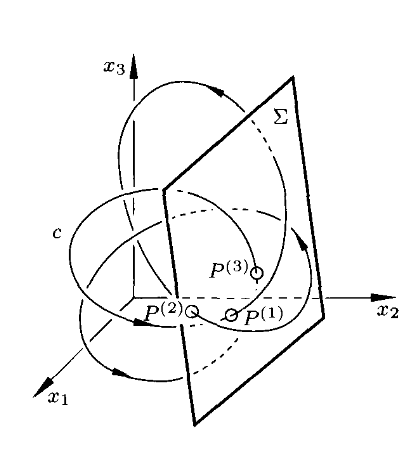
\includegraphics[scale=0.45]{images/poincare_cycle3.png}
    \end{center}

    \hfill
    \hrule
    \ \\
    {\footnotesize Bildquelle: An Exploration of Chaos, Argyris, Faus, Haase}
    }

    \only<2>
    {
    Poincaré-Bedingung:
    $$\theta_2 = 0, \quad \dot\theta_2 > 0$$

    \vfill

    Poincaré-Schnitt:
    \begin{enumerate}
    \item Wähle Parameter $l_1$, $l_2$, $m$, $g$
    \item Wähle Energie $E$
    \item Wähle Anfangsbedingungen $\theta_1(0)$, $\dot\theta_1(0)$
    \item Berechne numerisch $\theta_1(t)$, $\dot\theta_1(t)$, $\theta_2(t)$, $\dot\theta_2(t)$ und trage Punkt ins Plot ein, wenn $\theta_2(t)=0$
    \end{enumerate}
    }
}

\frame {
    \frametitle{Poincaré-Schnitt für $E=15$}

    \begin{center}
    \includegraphics[width=0.65\textwidth]{plots/E=15.pdf}
    \end{center}
}

\section{Beispiele}

\frame {
    \frametitle{Beispiel -- stabiler periodischer Orbit}

    \begin{center}
    \includemovie[poster,autoplay,controls=true]{7.5cm}{7.5cm}{videos/periodisch.mpeg}

    $E=15$, $\theta_1=0$, $p_1=2.63362868$
    \end{center}
}

\frame {
    \frametitle{Beispiel -- stabiler periodischer Orbit}

    \begin{center}
    \includemovie[poster,autoplay,controls=true]{7.5cm}{7.5cm}{videos/periodisch_kompliziert.mpeg}

    $E=15$, $\theta_1=0$, $p_1=-2.78854801$
    \end{center}
}

\frame {
    \frametitle{Beispiel -- instabiler periodischer Orbit}

    \begin{center}
    \includemovie[poster,autoplay,controls=true]{7.5cm}{7.5cm}{videos/periodisch_instabil.mpeg}

    $E=15$, $\theta_1=0$, $p_1=-4.10536235$
    \end{center}
}

\frame {
    \frametitle{Beispiel -- quasiperiodischer Orbit}

    \begin{center}
    \includemovie[poster,autoplay,controls=true]{7.5cm}{7.5cm}{videos/quasiperiodisch.mpeg}

    $E=15$, $\theta_1=0$, $p_1=-5$
    \end{center}
}

\frame {
    \frametitle{Beispiel -- Chaos}

    \begin{center}
    \includemovie[poster,autoplay,controls=true]{11cm}{5.5cm}{videos/chaos.mpeg}
    links: $E=15$, $\theta_1=0.8$, $p_1=-4$ \\
    rechts: $E=15$, $\theta_1=0.8$, $p_1=-4.01$
    \end{center}
}

\frame {
    \frametitle{Zusammenfassung}

    \begin{itemize}
        \item Vergleich verschiedener Anfangsbedingungen
        \item Reduktion der Dimension ohne Verlust an Informationen
        \item qualitatives Verhalten:
        \begin{itemize}
            \item Fixpunkte entsprechen periodische Orbits
            \item Unterscheidung chaotischer und regulärer Bereiche
            \item Linien entsprechen quasiperiodischer Orbits
        \end{itemize}
    \end{itemize}
}


\end{document}
